\documentclass[oneside]{book}
\usepackage[T1]{fontenc}
\usepackage{hyperref}
\hypersetup{
  linktocpage,
  colorlinks
}
\usepackage{soul}
\usepackage{inconsolata}
\renewcommand{\familydefault}{\sfdefault}

\usepackage{graphicx}
\usepackage[dvipsnames]{xcolor}
\usepackage{pdfpages}

\definecolor{base02}{HTML}{073642}
\definecolor{base00}{HTML}{839496}
\definecolor{orange}{HTML}{b58900}
\definecolor{cyan}{HTML}{2aa198}

\usepackage{parskip}
\setlength{\parindent}{0pt}
\setlength{\parskip}{4mm}

\usepackage{listings}
\usepackage[framemethod=tikz]{mdframed}
\usepackage[cm]{fullpage}


\lstdefinelanguage{Flex}{
  otherkeywords= {\%\%, \%\{, \%\}, \%option}
}


\lstloadlanguages{C,make}
\lstset{%
showstringspaces=false,
basicstyle=\ttfamily\color{base00},
commentstyle=\ttfamily\color{red},
keywordstyle=\ttfamily\color{orange},
identifierstyle=\ttfamily\color{base00},
stringstyle=\ttfamily\color{cyan}}

\surroundwithmdframed[
  hidealllines=true,
  fontcolor=base00,
  backgroundcolor=base02,
  innerleftmargin=15pt,
  innertopmargin=15pt,
  innerrightmargin=15pt,
  roundcorner=5pt,
  innerbottommargin=5pt]{lstlisting}


\date{}

\begin{document}
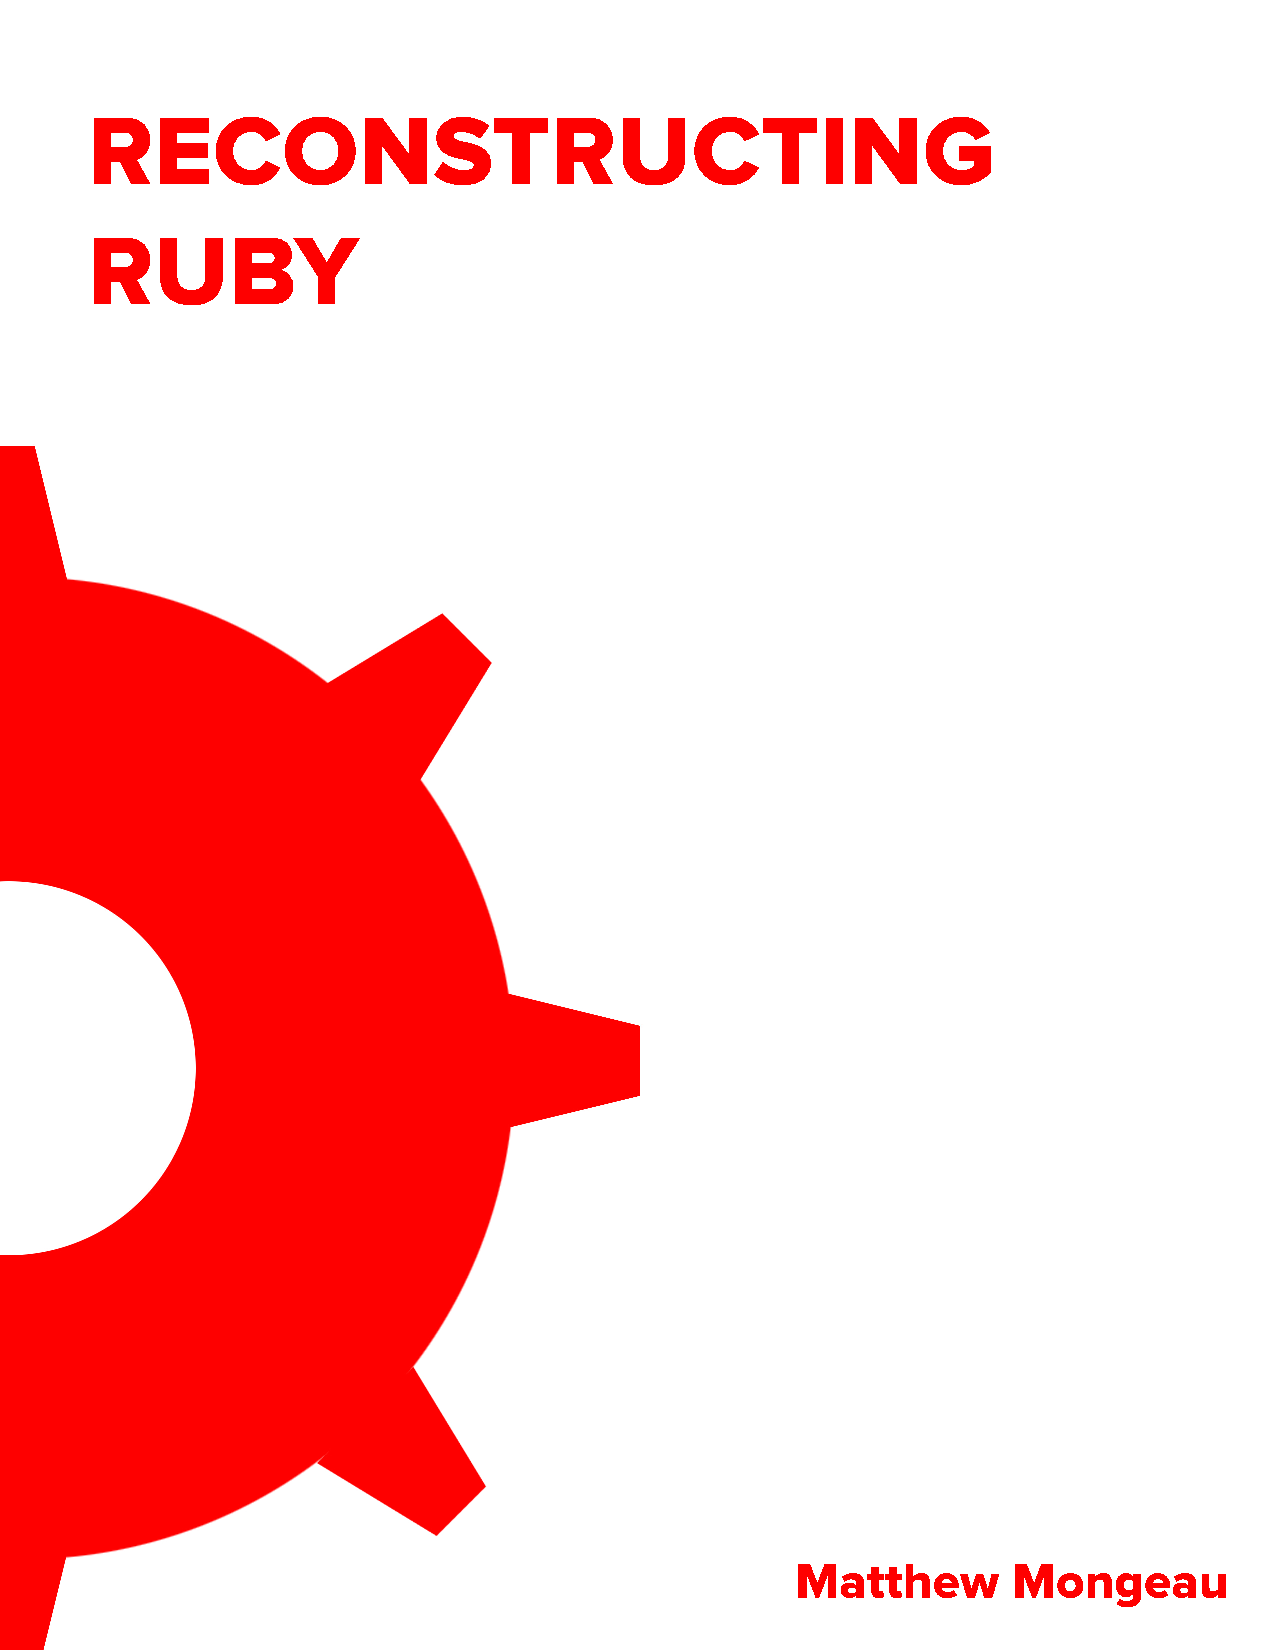
\includepdf{book/title.pdf}
\title{Reconstructing Ruby}
\author{Matthew Mongeau}
\maketitle

\frontmatter
\tableofcontents
\chapter*{Preface}
\addcontentsline{toc}{chapter}{Preface}

This book is not a primer on C. It assumes that you have a passing knowledge of C programming. If you've never programmed in C before it's highly suggested that you read the book "C Programming Language, 2nd Edition" by Brian W. Kernighan and Dennis M. Ritchie -  which is often referred to as "K\&R".

This book has been written for two purposes. The first is to provide a better understanding of Ruby's internals, potentially allowing readers to contribute to Ruby. A second goal is to provide a better understanding of interpreters in general. The second goal opens up the possibilities for readers to create their own interpreted languages.



\mainmatter
\chapter{Tokenizing}
What is a lexer? The job of a lexer is to read you code and identify what we call tokens. Tokens are simply named pieces of text. We'll be using a program called Flex to tokenize our code. Flex is a lexical analyzer designed to create a tokenizer.

A Flex file will typically have this structure:

\begin{lstlisting}
definitions and directives
%%
rules
%%
user code
\end{lstlisting}

As a first step we'll want to create a file called {\bf ruby.l}. Add the following content:

\begin{lstlisting}[language=C]
%{
  #include <stdlib.h>
  #include <stdio.h>
%}

%option noyywrap

%%
[0-9]+ { printf("NUMBER: %s\n", yytext); }
[ \t\n] {}
. {}
%%

int main(int argc, char *argv[]) {
  yylex();
  return EXIT_SUCCESS;
}
\end{lstlisting}

Now to compile and run this do the following

\begin{lstlisting}
flex ruby.l
gcc -o ruby lex.yy.c
./ruby
\end{lstlisting}

Then try the following:

\begin{lstlisting}
1
NUMBER: 1
42
NUMBER: 42
\end{lstlisting}

Then press ctrl-c to exit

\chapter{Parsing}
What is parsing? Parsing is verifying the structure of our code.



\appendix
\chapter{References}

\backmatter
\chapter{Notes}
\end{document}
